\chapter{Algoritmos}\label{chapter:algorithms}

\section{DP/DPLL}

\subsection{Principio de Resolución (PR)}
El Principio de Resolución (PR) es una de las primeras técnicas aplicadas para intentar resolver SAT.

Dada una fórmula de la Lógica Proposicional escrita en Forma Normal Conjuntiva (FNC), esta se representa en su forma conjuntual, donde cada cláusula constituye un conjunto de literales y la fórmula en general es un conjunto de conjuntos. Gracias al concepto de ``conjunto'' esta representación evita la repetición de literales en las cláusulas, así como aquellas que aparezcan más de una vez en la FNC. 

Tomando esta representación como entrada, PR busca iterativamente pares de clásulas que contengan literales opuestos, para a partir de ellas generar una nueva clásula que constituya la unión de ambas, quitando eliminando el literal en cuestión y su opuesto. Es decir:

Sean $\textbf{B}$ y $\textbf{C}$ dos cláusulas de la FNC $\textbf{A}$, tales que $l \in \textbf{B}$ y $\neg l \in \textbf{C}$, donde $l$ es un literal y $\neg l$ su opuesto; entonces la cláusula resultante sería:
\begin{equation*}
\textbf{D} = (\textbf{B}-\{l\}) \cup (\textbf{C}-\{\neg l\})
\end{equation*}

Aquí las cláusulas $\textbf{B}$ y $\textbf{C}$ se denominan ``cláusulas padres'' o ``premisas'' y $\textbf{D}$ constituye el ``solvente'' o ``conclusión'' de $\textbf{B}$ y $\textbf{C}$.

Téngase en cuenta el siguiente ejemplo para una mejor comprensión.

\begin{equation*}
\frac{\{\neg p, \neg q, \neg r\},\{\neg p, q, \neg r\}}{\{\neg p, \neg r\}}
\end{equation*}

\begin{equation*}
\frac{\{\neg q\},\{q\}}{\{\}}
\end{equation*}




El objetivo principal de PR es refutar $\textbf{A}$ si esta es insatisfacible, derivando una cláusula vacía ($\{\}$). Es decir, si $\{\} \in \textbf{A}$ entonces $\textbf{A}$ es insatisfacible, y si $\{\} = \textbf{A}$ entonces $\textbf{A}$ es satisfacible.

\subsubsection{Resolución Unitaria (RU)}
Un caso particular de PR es Resolución Unitaria (RU), donde una de las ``cláusulas padres'' es una cláusula unitaria \footnote{Cláusula que contiene un único literal, por ende su valor se ve forzado a ser 1.} Por ejemplo:

\begin{equation*}
\dfrac{\{\neg q, p, \neg r\},\{r\}}{\{\neg q, p\}}
\end{equation*}


\subsection{Davis-Putnam (DP)}
Uno de los primeros algoritmos para resolver SAT fue Davis-Putnam (DP), donde PR constituye uno de sus pilares. DP realiza tres procedimientos fundamentales: Propagación Unitaria (PU), Eliminación de Literales Puros (ELP) y Resolución Basada en División (RD). PU busca en la FNC de entrada clásulas unitarias y procede a eliminarlas de la fórmula, además de eliminar el literal complemntario de cada cláusula donde aparezca. ELP busca los literales que tengan una única polaridad en toda la fórmula (no exista su complementario) y procede a eliminar aquellas cláusula que contengan literales puros. Ambas, PU y ELP, son preprocesamientos que buscan simplificar lo más posible la FNC. Una vez realizados, DP procede con RD donde asigna un valor (0 o 1) a una variable y continúa recursivamente aplicando DP hasta encontrar poder decidir si la FNC es satisfacible o no. Véase el ejemplo a continuación:

Sean las siguientes, fórmulas de la Lógica Proposicional

\begin{equation*}
r, [q \land r] \implies p, [q \lor r ] \implies \neg p, [\neg q \land r] \implies \neg p, \neg s \implies p
\end{equation*}


A paritr de la conjunción de estas, se obtiene la siguiente FNC:

\begin{equation*}
{\{r\}, \{p,\neg q, \neg r\}, \{\neg p, \neg q\}, \{\neg p, \neg r\}, \{\neg p,q,\neg r\}, \{p,s\}}
\end{equation*}

Aplicando \textbf{PU} en $\{r\}$:

\begin{equation*}
\{\{p,\neg q\},\{\neg p,\neg q\},\{\neg p\},\{\neg p,q\},\{p,s\}\}
\end{equation*}

Aplicando \textbf{PU} en $\{\neg p\}$:

\begin{equation*}
\{\{\neg q\},\{s\}\}
\end{equation*}

Aplicando \textbf{PU} en $\{\neg q\}$:

\begin{equation*}
\{\{s\}\}
\end{equation*}

Aplicando \textbf{PU} en $\{s\}$:

\begin{equation*}
\{\}
\end{equation*}

Luego la fórmula es satisfacible.

DP requiere una memoria exponencial ya que evalúa todas las posibles asignaciones para las variables, generando un árbol de decisión como espacio de búsqueda que crece exponencialmente.

\begin{figure}[ht]
    \centering
    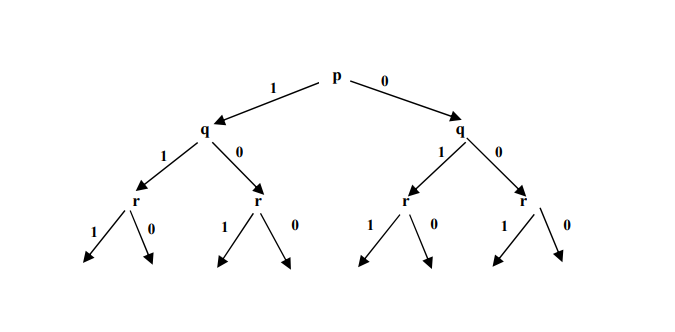
\includegraphics[width=0.8\textwidth]{Graphics/arboldp.png}
    \caption{Posible espacio de búsqueda de una FNC}
    \label{fig:arbol DP}
\end{figure}

\subsection{Davis-Putnam-Logemann-Loveland (DPLL)}
El algoritmo Davis-Putnam-Logemann-Lovelans (DPLL) aplica las mismas bases que DP, excepto que resuelve el problema de la memoria exponencial al realizar un \textit{backtrack} cronológico (al nivel anterior de decisión) en el árbol de asignaciones una vez encontrada una ``cláusula de conflicto''\footnote{Se denomina cláusula de conflicto a aquella cláusula cuyos literales evaluaron a 0 tras una asignación.}. Con este método, DPLL utiliza una estrategia \textit{``lazy''} para generar el árbol, dado que antes de ramificarse (otorgar un valor a una variable) verifica que no haya conflictos, garantizando que las asiganaciones válidas para la fórmula de entrada se encuentren en las hojas del árbol de decisión. Obsérvese que si un conflicto se produce en el nivel de decisión 0 y ambos valores para la variable ya han sido examinados, entonces se concluye que la fórmula es insatisfacible. Este proceso realizado por DPLL se denomina ramificación + propagación unitaria + retroceso.

Cabe destacar que DPLL tiene una etapa de preprocesamiento de la FNC, sobre la cual se aplican leyes de la Lógica Proposicional, así como se eliminan cláusulas redundantes mediante la aplicación de la subsunción de cláusulas\footnote{Sean $C$ y $C'$, cláusulas de una FNC; si $C' \subseteq C$, entonces se elimina $C'$ de la FNC.}. 

Obsérvese el siguiente ejemplo:

Sea la FNC:

\begin{equation*}
\{\{\neg p,\neg q\},\{\neg p, \neg q\},\{\neg p,q,\neg r\},\{\neg p,r,s\},\{p,s\}\}
\end{equation*}

Simplificando mediante la Ley de Absorción:

\begin{equation*}
\{\{\neg p,\neg q\},\{\neg p,q,\neg r\},\{\neg p,r,s\},\{p,s\}\}
\end{equation*}

Eliminando el literal puro $s$:

\begin{equation*}
\{\{\neg p,\neg q\},\{\neg p,q,\neg r\}\}
\end{equation*}

Ramificando: $p=1$

\begin{equation*}
\{\{\neg q\},\{q,\neg r\}\}
\end{equation*}

Aplicando PU:

\begin{equation*}
\{\{\neg q\},\{q,\neg r\}\}
\end{equation*}

Aplicando PU:

\begin{equation*}
\{\neg r\}
\end{equation*}

\begin{equation*}
\emptyset
\end{equation*}


Luego la FNC es satisfacible.

No obstante la reducción del espacio de memoria de DPLL respecto a DP, aún quedan problemas fundamentales: selección de variables, \textit{backtrack} cronológico y selección de cláusulas unitarias.

En primer lugar la selección de la variable a asignar un valor influye en la ``forma'' que tomará el espacio de búsqueda, por lo que malas decisiones en este sentido conllevan a caminos más largos en la búsqueda de una solución. Análogamente se gana en eficiencia considerando heurísticas en la selección de variables. (poner ejemplo)

En segundo lugar, el \textit{backtrack} cronológico a partir de un conflicto obliga a explorar el resto de las posibles asignaciones de las variables en niveles anterirores, potencialmente, de forma innecesaria, sobre todo para aquellos casos donde la asignación causante del conflicto se encuentre a $k$ niveles de distancia del nivel del conflicto. Además, DPLL no aprovecha las cláusulas que han resultado conflictos, es decir, no aprende de ellas, por lo que es vulnerable a cometer el mismo error (mismo patrón incorrecto de asignaciones para las variables involucradas en el conflicto). Esto lo hace susceptible a repetir errores de forma recurrente.

Finalmente, el problema de selección de cláusulas unitarias, influye también en la eficiencia del algoritmo. Se puede decir que guarda relacón con la estrategia de selección de variables.

\section{CDCL}
CDCL es una mejora que se le añadió al algoritmo DPLL con el objetivo de erradicar el problema del retroceso (\textit{backtrack}) cronológico, una vez encontrada una cláusula de conflicto (todos sus literales evalúan 0).

El retroceso cronológico consiste en recorrer el árbol de decisión (estructura propia del algoritmo DPLL que se forma al asignarle valores a las variables) retrocediendo de a 1 por cada nivel, probando todos los valores aún sin explorar de cada variable hasta encontrar la asignación causante del conflicto. Esta búsqueda es ineficiente dado que, además de analizar casos innecesarios, se vuelve susceptible a cometer el mismo error en el futuro (potencialmente realiza la misma combinación de asignaciones) generando búsquedas redundantes.

Para solucionar este problema, CDCL crea un grafo dirigido y acíclico que permite guardar el historial de asignaciones de cada variable. En dicho grafo, los nodos son las variables y los arcos constituyen la causa de la asignación de dicha variable: la cláusula a la que pertenece, si fue asignada por propagación unitaria, y null para variables asignadas por decisión. El grafo también contiene 2 metadatos: el valor asignado a cada variable (0 o 1), y el nivel de decisión en el que se asignó (los diferentes niveles de decisión están marcados por la asignación de valores por decisión). Cabe destacar que la dirección de los arcos en el grafo va desde las variables de decisión hacia aquellas que, en el mismo nivel, tuvieron que forzar su valor por propagación unitaria. En el caso de una nueva variable de decisión, se crea un nuevo arco con valor nulo desde la variable asignada por decisión en el nivel anterior, hasta la nueva variable.

Cuando una cláusula resulta ser de conflicto (sus literales evaluaron 0), CDCL crea un nuevo nodo en el grafo que representa dicho conflicto, para comenzar con su análisis.
Este análisis busca en el grafo la asignación causante del conflicto, para retroceder justo hacia ese punto y realizar un \textit{backjump} en lugar de un retroceso cronológico, como en DPLL. Asimismo, con este análisis CDCL busca conformar una cláusula (cláusula aprendida) que represente la combinación de asignación de valores que condujo a dicho conflicto, para incluirla en la base de datos de las cláusulas de la FNC y evitar cometer el mismo error en iteraciones futuras. El punto escogido para realizar el \textit{backjump} es conocido como primer punto de implicación único (\textit{First-UIP} por sus siglas en inglés). Este punto, será aquel literal que en la cláusula aprendida, posea el más alto nivel de decisión, diferente del actual.

Es necesario enfatizar en el hecho de que la cláusula aprendida debe contener únicamente 1 literal cuyo valor haya sido asignado en el nivel de decisión actual. En caso de haber más de uno, CDCL recorre el grafo en busca de la cláusula que causó la asignación de una de estas variables y aplica el Principio de Resolución entre esta y la cláusula aprendida hasta el momento. La cláusula resultante pasará a ser la nueva cláusula aprendida. El proceso se repetirá hasta que la cláusula aprendida contenga solo un literal cuyo valor fue asignado en el nivel de decisión actual.

En caso de que el nivel del \textit{backjump} sea el nivel 0, CDCL considera la FNC como insatisfacible.

A continuación, se muestra como ejemplo la implementación en Python de un CDCL SAT \textit{solver}

\begin{lstlisting}
class SATSolver:
    def __init__(self, formula):
        """
        Initializes the SAT solver.
        
        Parameters:
          formula: A list of clauses, where each clause is represented as a list of integers.
                   A positive integer i represents the variable x_i, and a negative integer -i represents -x_i.
        """
        # Copy the formula so that learned clauses can be appended.
        self.formula = formula[:]  
        self.assignments = {}    # Maps variable -> True/False assignment.
        self.levels = {}         # Maps variable -> decision level at which it was assigned.
        self.reasons = {}        # Maps variable -> clause that forced the assignment (None for decision variables).
        self.decision_level = 0  # Current decision level.
        self.decision_stack = [] # Stack storing tuples (variable, assigned value, decision level).

    def literal_value(self, literal):
        """
        Evaluates a literal given the current partial assignment.
        
        Returns:
          True if the literal is assigned True,
          False if the literal is assigned False,
          None if the variable is unassigned.
        """
        var = abs(literal)
        if var not in self.assignments:
            return None
        # For a positive literal, the assignment is the value; for a negative literal, invert the assignment.
        return self.assignments[var] if literal > 0 else not self.assignments[var]

    def check_clause(self, clause):
        """
        Determines the status of a clause with respect to current assignments.
        
        Returns a tuple (status, literal) where status is one of:
          - `satisfied': Clause is already True under the assignment.
          - `conflict': All literals are assigned False (the clause is unsatisfied).
          - `unit': Exactly one literal is unassigned while all others are False (this literal must be True).
          - `undefined': The clause is neither satisfied, conflicting, nor unit.
        """
        satisfied = False
        unassigned_count = 0
        unit_literal = None
        for literal in clause:
            val = self.literal_value(literal)
            if val is True:
                return (`satisfied', None)
            if val is None:
                unassigned_count += 1
                unit_literal = literal  # Last seen unassigned literal.
        if unassigned_count == 0:
            return (`conflict', None)
        if unassigned_count == 1:
            return (`unit', unit_literal)
        return (`undefined', None)

    def unit_propagate(self):
        """
        Repeatedly applies unit propagation.
        
        Returns:
          A conflicting clause if a conflict is found during propagation; otherwise, returns None.
        """
        changed = True
        while changed:
            changed = False
            for clause in self.formula:
                status, unit_literal = self.check_clause(clause)
                if status == 'conflict':
                    # A clause is unsatisfied => conflict!
                    return clause
                elif status == `unit':
                    var = abs(unit_literal)
                    if var not in self.assignments:
                        # Determine the value needed to satisfy the unit clause.
                        value = (unit_literal > 0)
                        self.assignments[var] = value
                        self.levels[var] = self.decision_level
                        self.reasons[var] = clause  # Store the clause as the reason for this assignment.
                        self.decision_stack.append((var, value, self.decision_level))
                        changed = True
        return None

    def pick_branching_variable(self):
        """
        Selects the next unassigned variable found in the formula.
        
        (In a production solver, better heuristics like VSIDS are used.)
        """
        variables = set()
        for clause in self.formula:
            for literal in clause:
                variables.add(abs(literal))
        for var in variables:
            if var not in self.assignments:
                return var
        return None

    def resolve(self, clause1, clause2, pivot):
        """
        Performs the resolution on two clauses over the pivot literal.
        
        Specifically, it returns:
          (clause1 \ {pivot}) U (clause2 \ {-pivot})
        """
        new_clause = []
        for lit in clause1:
            if lit == pivot:
                continue
            if lit not in new_clause:
                new_clause.append(lit)
        for lit in clause2:
            if lit == -pivot:
                continue
            if lit not in new_clause:
                new_clause.append(lit)
        return new_clause

    def conflict_analysis(self, conflict_clause): 
        """
        Conducts conflict analysis to find the First UIP.
        """
        learned_clause = conflict_clause.copy()
        current_level = self.decision_level

        while True:
            # Collect literals in the learned clause assigned at the current level
            current_level_lits = [
                lit for lit in learned_clause 
                if self.levels.get(abs(lit), -1) == current_level
            ]
            if len(current_level_lits) <= 1:
                break

            # Find the most recently assigned literal in current_level_lits
            last_literal = None
            # Iterate through assignments in reverse order (most recent first)
            for var, _, lvl in reversed(self.decision_stack):
                if lvl != current_level:
                    continue
                # Check if this variable is in current_level_lits
                for lit in current_level_lits:
                    if abs(lit) == var:
                        last_literal = lit
                        break
                if last_literal is not None:
                    break

            if last_literal is None:
                break  # No resolvable literals (should not happen)

            # Resolve with the reason clause of last_literal
            reason_clause = self.reasons.get(abs(last_literal))
            if reason_clause is None:
                break  # Decision literal; cannot resolve further

            learned_clause = self.resolve(learned_clause, reason_clause, last_literal)

        # Determine the backjump level
        backjump_level = 0
        for lit in learned_clause:
            lvl = self.levels.get(abs(lit), 0)
            if lvl != current_level and lvl > backjump_level:
                backjump_level = lvl

        return learned_clause, backjump_level

    def backjump(self, level):
        """
        Backtracks the search to the given decision level by undoing assignments above that level.
        """
        new_stack = []
        for var, value, lvl in self.decision_stack:
            if lvl > level:
                if var in self.assignments:
                    del self.assignments[var]
                if var in self.levels:
                    del self.levels[var]
                if var in self.reasons:
                    del self.reasons[var]
            else:
                new_stack.append((var, value, lvl))
        self.decision_stack = new_stack

    def solve(self):
        """
        The main solving loop which alternates between unit propagation, conflict analysis, and branching.
        
        Returns:
          A satisfying assignment as a dictionary mapping variables to Boolean values if the formula is SAT;
          Otherwise, returns None indicating the formula is UNSAT.
        """
        while True:
            conflict = self.unit_propagate()
            if conflict:
                if self.decision_level == 0:
                    # Conflict at level 0 indicates an unsolvable (UNSAT) condition.
                    return None
                learned_clause, backjump_level = self.conflict_analysis(conflict)
                # Learn the clause by adding it to the formula.
                self.formula.append(learned_clause)
                # Backjump to the appropriate decision level.
                self.backjump(backjump_level)
                self.decision_level = backjump_level
            else:
                var = self.pick_branching_variable()
                if var is None:
                    return self.assignments
                self.decision_level += 1
                # For this example, we simply decide that the variable is True.
                self.assignments[var] = True
                self.levels[var] = self.decision_level
                self.reasons[var] = None  # Decision assignments have no reason clause.
                self.decision_stack.append((var, True, self.decision_level))
\end{lstlisting}

La implementación anterior consiste en una clase SATSolver que realiza los pasos de CDCL dada una FNC escrita en forma de \textit{array} de \textit{arrays} donde estos últimos son las cláusulas. Por su parte, cada variable está representada por un número entero positivo y sus literales serán el propio número y su opuesto.

El primer método inicializa las estructuras con las que trabajará:
\begin{itemize}
\item \textit{assigments}: Mapea cada variable asignada con su valor.
\item \textit{levels}: Mapea cada variable aasignada con el nivel de decisión en el que se le dio su valor.
\item \textit{reasons}: Estos serán los ``arcos'' del grafo de decisión, pues mapea por cada variable asignada la cláusula que provocó su asignación, y \textit{None} para el caso de variables asignadas por decisión.
\item \textit{decision\_level}: guarda el actual nivel de decisión.
\item \textit{decision\_stack}: registra el grafo al guardar en una pila tuplas de 3 elementos: variable asignada, valor que tomó y el nivel de decisión en el que se le asignón su valor.
\end{itemize}

El bucle principal del algoritmo se encuentra en el método \textit{solve(self)} que mientras no haya conflicto asigna valores a las variables y actualiza las estructuras de la clase, y en caso de no existir más variables por asignar, entonces devuelve la solución (asignaciones para cada variable) declarando la fórmula como satisfacible. En cambio, si una cláusula conflicto es detectada y el nivel actual de decisión es 0, entonces devuelve \textit{None}, declarando no existe una asignación válida para las variables, luego la fórmula es insatisfacible.

El método encargado de realizar la propagación unitaria por cada nivel de decisión es \textit{unit\_propagate(self)}. Este, cosiste en un algoritmo de punto fijo que se ejecuta mientras haya cambio, es decir, mientras existan cláusulas unitarias, y en caso de haber una cláusula conflicto detiene el bucle y devuelve dicha cláusula. En caso de no haber conflicto, retorna \textit{None}. La salida de este algoritmo es tomada por el método \textit{solve()} explicado anteriormente. El status de una cláusula (`\textit{satisfied}', `\textit{conflict}', `\textit{unit}', `\textit{undefined}') es determinado por \textit{check\_clause(self, clause)}.

Una vez encontrada una cláusula de conflicto, se llama al método \textit{conflict\_analysis(self, conflict\_clause)}, el cual primero analiza a cuántas variables en la cláusula conflicto se le asignaron valor en el nivel de decisión actual. Esto debido a que la cláusula aprendida solo debe contener un literal cuyo valor haya sido asignado en el nivel de decisión actual. En caso de haber más de 1, se busca el último de estos literales cuya variable fue asignada, se toma a partir del grafo de decisión la cláusula que causó su asignación, y se realiza Pincipio de Resolución con esta y la actual cláusula aprendida. La cláusula resultante para a ser la cláusula aprendida hasta el momento. Este prcedimiento se repite hasta que solo quede un literal asignado en el actual nivel de decisión.

Luego de obtener la cláusula aprendida a partir de un conflicto se determina el \textit{backjump level}, el cual será el nivel de decisión más alto de los literales se la cláusula aprendida. Una vez hallado el nivel al cual retroceder, el método \textit{backjump(self, level)} realiza las actualizaciones de todas las estructuras de la clase (\textit{backjump}).


\section{DLIS}
La heurística Dynamic Largest Individual Sum (DLIS) para selección de variables, es uno de los métodos aproximados que pueden integrarse en un CDCL SAT \textit{solver} con el objetivo de aumentar la eficiencia al asignar un valor a una variable en cada nivel de decisión.

DLIS lleva un contador por cada variable que indica el número máximo que clásulas insatisfechas que pueden resolverse al asignar uno de los dos valores (0 o 1). Es decir, dada una variable $x$, se calcula la cantidad de cláusulas insatisfechas en las que aparece el literal $x$ y su complementario $\neg x$. Sea $dlis(x)$ la mayor cantidad de cláusulas que $x$ puede satisfacer, y $count_pos(x)$ y $count_neg(x)$ la cantidad de veces que aparece el literal positivo y negativo, repectivamente, en cláusulas aún sin resolver; luego:

\begin{equation*}
dlis(x)=max(count_pos(x), count_neg(x))
\end{equation*}

Teniendo en cuenta este cálcula la próxima variable a asignar será:
\begin{equation*}
x_k \mid dlis(x_k)=max(dlis(x_i)), i \in [1,n]
\end{equation*}

donde $n$ es la cantidad de variables de la FNC.

Obsétvese que si $count_pos(x_k) > count_neg(x_k)$ entonces $x_k$ tomará como valor 1, y 0 en caso contrario, puesto que el objetivo es satisfacer dichas cláusulas. Téngase en cuenta que el cálculo se le aplica a las variables que aún no han sido asignadas, además de solo tenerse en cuenta aquellos valores que aún no han sido explorados para una misma variable en el actual nivel de decisión.

La estrategia de selección de variables se puede insertar en el anterior algoritmo de CDCL en el método \textit{pick\_branching\_variable(self)} el cual se encarga de decidir la próxima variable a la cual se le asignará un valor (0 o 1). Tomando como base el código anterior y modificando el método \textit{pick\_branching\_variable(self)}, una posible implementación de DLIS podría quedar de la siguiente forma:

\begin{lstlisting}
def pick_branching_variable(self):
    """
    Selects the next unassigned variable using the DLIS heuristic.
    Returns (variable, value) to assign, or None if all variables are assigned.
    """
    pos_counts = {}
    neg_counts = {}
    # Count occurrences in unsatisfied clauses
    for clause in self.formula:
        status, _ = self.check_clause(clause)
        if status == 'satisfied':
            continue
        for lit in clause:
            var = abs(lit)
            if var not in self.assignments:
                if lit > 0:
                    pos_counts[var] = pos_counts.get(var, 0) + 1
                else:
                    neg_counts[var] = neg_counts.get(var, 0) + 1
    # Collect all variables in the formula to find unassigned ones not in any clause
    all_vars = set()
    for clause in self.formula:
        for lit in clause:
            all_vars.add(abs(lit))
    unassigned_vars = [var for var in all_vars if var not in self.assignments]
    if not unassigned_vars:
        return None
    # For variables not in pos/neg counts, set counts to 0
    for var in unassigned_vars:
        if var not in pos_counts:
            pos_counts[var] = 0
        if var not in neg_counts:
            neg_counts[var] = 0
    # Score variables based on DLIS heuristic
    scores = []
    for var in unassigned_vars:
        pos = pos_counts[var]
        neg = neg_counts[var]
        max_count = max(pos, neg)
        total = pos + neg
        scores.append((-max_count, -total, var))  # Negative for ascending sort
    scores.sort()  # Sorts by max_count (desc), then total (desc), then var (asc)
    var = scores[0][2]
    value = pos_counts[var] > neg_counts[var]
    return (var, value)

\end{lstlisting}

Las estructuras \textit{pos\_counts} y \textit{neg\_counts} almacenan la cantidad de veces que el literal positivo y el negativo, respectivamente, de una variable aparece en cláusulas aún sin satisfacer. Para actualizar estas estructuras primero se inspeccionan aquellas cláusulas que aún no han sido resueltas. Luego se completa la información con aquellas variables sin asignar que no se hayan incluido en el procedimiento anterior y se pone su contador en 0. Este puede ser el caso de variables sin asignar que solo se encuentren en cláusulas satisfechas (a otra variable de la misma cláusula se le asignó 1 como valor). Una vez actualizado el conteo por cada literal, se haya el \textit{score} por vaiable (el máximo entre ambos conteos), se ordenan de mayor a menor y se decide asignar aquella variable con el \textit{score} más alto. El valor a asignársele a esta variable es el de mayor conteo entre ambas polaridades.

Con esta estrategia DLIS busca satisfacer en una sola asignación la mayor cantidad de cláusulas posibles, sin embargo, esta estrategia resulta costosa en instancias grandes: $O(n)$ por cada nivel de decisión, donde $n$ es la cantidad de literales.

\section{VSIDS}
Por su parte, la heurística Variable State Independent Decaying Sum (VSIDS) prioriza asignarle valores aquellas variables que hayan estado en conflictos recientes. Para ello, VSIDS lleva un \textit{score} por cada literal $l$ (no por cada variable) que aumenta cada vez que aparezcan en clásulas aprendidas de conflictos. Además, para evitar que literales que hayan pertenecido a conflictos pasados y no recientes sean tenidos en cuenta por encima de los más actuales, cada cierta cantidad $T$ de conflictos se multiplica los \textit{scores} de cada literal por $\alpha$, donde $0 < \alpha < 1$ (usualmente $\alpha = 0.95$). Integrado con CDCL, VSIDS se comportaría de la siguiente forma:
\begin{enumerate}
    \item Procede el algoritmo CDCL.
    \item Si ocurre un conflicto, se añade la cláusula aprendida $\mathbf{C_{learn}}$. Luego, por cada literal $l$ tal que $l \in \mathbf{C_{learn}}$ se tiene que $score(l) += \delta$, donde $\delta$ es el incremento.
    \item Si ocurre el conflicto $T$-ésimo, entonces $\delta = \delta \cdot \alpha$ con $0 < \alpha < 1$.
    \item Si no ocurre un conflicto, se seleccionará según VSIDS la variable $v$ si $score(l_v) = \max(score(l_i))$ para todo $i$ tal que $1 \leq i \leq 2n$, con $n$ cantidad de variables. Si $l_v$ es positivo, entonces $v$ tomará valor 1, y 0 en caso contrario.
\end{enumerate}

Una posible implementación para VSIDS que se integre al código base anterior de CDCL es la siguiente.

\begin{lstlisting}
def pick_branching_variable(self):
    """
    Selects the next unassigned variable using the VSIDS heuristic (highest activity).
    """
    candidates = []
    for var in self.activity:
        if var not in self.assignments:
            candidates.append(var)
    if not candidates:
        return None
    # Select the candidate with the highest activity; in case of tie, choose the smallest variable.
    max_activity = max(self.activity[var] for var in candidates)
    best_vars = [var for var in candidates if self.activity[var] == max_activity]
    best_vars.sort()  # Deterministic tie-breaking by choosing the smallest variable
    return best_vars[0]
\end{lstlisting}

Este método solo selecciona entre las que no han sido asignadas, aquella variable con mayor \textit{score} de acuerdo al criterio de este algoritmo. Para llevarlo a cabo, se añadió a la clase \textit{SATSolver} una estructura \textit{activity} que mapea cada variable con su \textit{score}. Esta estructura se inicializaría como se muestra a continuación:

\begin{lstlisting}
# previus code
    for clause in self.formula:
        for lit in clause:
            var = abs(lit)
            if var not in self.activity:
                self.activity[var] = 0.0
\end{lstlisting}

Además, \textit{activity} se pudiese actualizar dentro del método \textit{solve(self)} de la siguiente forma:

\begin{lstlisting}
decay_factor = 0.95
while True:
           conflict = self.unit_propagate()
           if conflict:
               if self.decision_level == 0:
                    # Conflict at level 0 indicates an unsolvable (UNSAT) condition.
                   return None
               learned_clause, backjump_level = self.conflict_analysis(conflict)
               # Learn the clause by adding it to the formula.
               self.formula.append(learned_clause)
               # Update activities for variables in the learned clause
               for lit in learned_clause:
                   var = abs(lit)
                   self.activity[var] += 1.0
               # Decay all activities
               for var in self.activity:
                   self.activity[var] *= decay_factor
               # Backjump to the appropriate decision level.
               self.backjump(backjump_level)
               self.decision_level = backjump_level
# rest of code
\end{lstlisting}

\section{Reinicio (\textit{restart})}
Las estrategias de reinicio buscan no estancarse en espacios locales de búsqueda mediante un ``reinicio'' del árbol de decisión, es decir, eliminan todas las asignaciones realizadas hasta el momento y vuelven a empezar, pero manteniendo en la FNC las cláusulas aprendidas producto de CDCL, y los datos extras como \textit{scores} de los literales que hayan aportado las heurísticas de selección de variables.

Existen varios criterios para realizar los \textit{restarts}:
\begin{enumerate}
\item Fijo: se reinicia cada $k$ conflictos fijos.
\item Geométrico: cada intervalo $r_i$ crece como un secuencia geométrica de la siguiente forma: $r_0 = b; r_i = \alpha \cdot r_{i-1} \mid \alpha > 1$. Es importante definir bien el valor de $\alpha$ pues si este es muy grande los reinicios serán muy espaciados, y si es muy pequeño habrá una sobrecarga de \textit{restarts}.
\item Luby: Este reinicio se basa en la secuencia de Luby (1,1,2,1,1,2,4,1,1,2,…), obteniéndose que $r_i = b \cdot Luby(i)$, donde $r_i$ constituye el i-ésimo \textit{restart}, y $b$ es un parámetro de intervalo.
\item \textit{Glucose-style (LBD-based)}: esta estrategia está basada en el cálculo Literal Block Distance (LBD) que consiste en, dada una cláusula aprendida, contar la cantidad de niveles de decisión diferentes a los que pertenecen cada uno de sus literales. Es decir, dada una cláusula aprendida $C_{learm}$ se tiene que $LBD(C_{learn}) = \|\{level(l)\: l \in C_{learn} \}\|$. LBD busca medir la calidad de una cláusula a partir de la diversidad de niveles de decisión en una cláusula, planteando que mientras menor sea este número las variables implicadas en el conflicto estarán más cerca en el árbol de decisión, por ende más relacionadas, luego más útil la cláusula. Por tanto, a menor LBD, mayor calidad de cláusula. Ahora, la estrategia de reinicio \textit{Glucose-style} haya dos promedios de LBD para una ventana ``rápida'' (usualmente 50 o 100 últimos conflictos) y una ventana ``lenta'' (usualmente 1000 últimos confilctos)de cantidad de conflictos. Estas dos cantidades se dividen de la siguiente forma: sean $\mu_r$ promedio de LBD en la ventana rápida de últimos conflictos, y $\mu_l$ su homólogo para la ventana lenta; sea, además, $T > 1$ umbral de decisión, entonces \textit{Glucose-style} realiza la comparación $\dfrac{\mu_r}{\mu_l} > T$, y si esta resulta verdadera entonces procede con el reinicio. Esta estrategia sugiere que si el promedio de LBD en cláusulas aprendidas recientes supera significativamente al de cláusulas más antiguas, el algoritmo estaría estancado en espacios locales de búsqueda infructíferos.
\end{enumerate}

Ussando como base el código anterior de CDCL, una posible implementación para la estrategia Luby puede ser la siguiente:

\begin{lstlisting}
# restart_luby.py

from collections import deque

def luby(u, k):
    """
    Generates the k-th value of the Luby sequence multiplied by u (unit run).
    """
    def _luby(i):
        # Encuentra el mayor j tal que i = 2^j - 1
        j = 1
        while (1 << j) - 1 < i:
            j += 1
        if i == (1 << j) - 1:
            return 1 << (j - 1)
        return _luby(i - (1 << (j - 1)) + 1)
    return u * _luby(k)

class SATSolverLuby:
    def __init__(self, formula, unit_run=100):
        from restart_luby import luby  # si ejecutas desde fuera
        self.formula = formula[:]  
        self.assignments = {}
        self.levels = {}
        self.reasons = {}
        self.decision_level = 0
        self.decision_stack = []
        # Luby restart parameters
        self.unit_run = unit_run
        self.luby_idx = 1
        self.conflicts_since_restart = 0
        self.next_restart = luby(self.unit_run, self.luby_idx)

    # the same functions (literal_value, check_clause, unit_propagate,
    # pick_branching_variable, resolve, conflict_analysis, backjump)

    def solve(self):
        while True:
            conflict = self.unit_propagate()
            if conflict:
                self.conflicts_since_restart += 1
                if self.decision_level == 0:
                    return None
                learned_clause, backjump_level = self.conflict_analysis(conflict)
                self.formula.append(learned_clause)
                self.backjump(backjump_level)
                self.decision_level = backjump_level

                # restart?
                if self.conflicts_since_restart >= self.next_restart:
                    # Restart: clear assignments, preserve learned clauses
                    self.assignments.clear()
                    self.levels.clear()
                    self.reasons.clear()
                    self.decision_stack.clear()
                    self.decision_level = 0
                    # Prepare next umbral
                    self.luby_idx += 1
                    self.next_restart = luby(self.unit_run, self.luby_idx)
                    self.conflicts_since_restart = 0
            else:
                var = self.pick_branching_variable()
                if var is None:
                    return self.assignments
                self.decision_level += 1
                self.assignments[var] = True
                self.levels[var] = self.decision_level
                self.reasons[var] = None
                self.decision_stack.append((var, True, self.decision_level))
\end{lstlisting}

Análogo a las heurísticas anteriores, se añaden nuevas estructuras a la clase \textit{SATSolver}, y en base a la estrategia de \textit{restart} de Luby, se decide en el método \textit{solve(self)} si es necesario un reinicio.

De igual modo, una implementación para la estrategia \textit{Glucose-Style (LBD-based)} sería como la que se muestra a continuación:

\begin{lstlisting}
# restart_glucose.py

class SATSolverGlucose:
    def __init__(self, formula, lbd_window=50):
        self.formula = formula[:]  
        self.assignments = {}
        self.levels = {}
        self.reasons = {}
        self.decision_level = 0
        self.decision_stack = []
        # Glucose-style parameters
        self.lbd_history = []
        self.window_size = lbd_window
        self.prev_avg_lbd = float('inf')

    #same base functions: literal_value, check_clause, unit_propagate, pick_branching_variable, resolve, backjump

    def conflict_analysis(self, conflict_clause):
        learned_clause, backjump_level = super().conflict_analysis(conflict_clause)
        # Calcular LBD (Literal Block Distance)
        levels = { self.levels.get(abs(l), 0) for l in learned_clause }
        lbd = len(levels)
        # Mantener ventana de LBDs
        self.lbd_history.append(lbd)
        if len(self.lbd_history) > self.window_size:
            self.lbd_history.pop(0)
        return learned_clause, backjump_level

    def should_restart(self):
        if len(self.lbd_history) < self.window_size:
            return False
        curr_avg = sum(self.lbd_history) / len(self.lbd_history)
        # Reiniciar si la media de LBD sube respecto al ciclo anterior
        if curr_avg > self.prev_avg_lbd:
            self.prev_avg_lbd = curr_avg
            return True
        self.prev_avg_lbd = curr_avg
        return False

    def solve(self):
        while True:
            conflict = self.unit_propagate()
            if conflict:
                if self.decision_level == 0:
                    return None
                learned_clause, backjump_level = self.conflict_analysis(conflict)
                self.formula.append(learned_clause)
                self.backjump(backjump_level)
                self.decision_level = backjump_level

                # Glucose-style restart
                if self.should_restart():
                    self.assignments.clear()
                    self.levels.clear()
                    self.reasons.clear()
                    self.decision_stack.clear()
                    self.decision_level = 0

            else:
                var = self.pick_branching_variable()
                if var is None:
                    return self.assignments
                self.decision_level += 1
                self.assignments[var] = True
                self.levels[var] = self.decision_level
                self.reasons[var] = None
                self.decision_stack.append((var, True, self.decision_level))

\end{lstlisting}

\section{Selección de cláusulas unitarias}

Una de las estrategias más usadas actualmente es \textit{Two Watched Literals (TWL)}. Esta tiene por objetivo evitar el recorrido de todas las cláusulas en el momento de realizar la propagación unitaria mediante la ``vigilancia'' de dos literales $l_1$ y $l_2$ por cada cláusula. Si durante el algoritmo tanto $l_1$ como $l_2$ no han sidp evaluados, pues no es necesario revisar dicha cláusula dado que no es unitaria ni de conflicto. En cambio, si alguno ha sido asignado a 0 se busca en cada cláusula otro literal para sustituirlo y, de no ser posible implicaría que la cláusula es unitaria (asumiendo que el otro literal vigilado no tiene valor). Si ambos literales son evaluados a 0, entonces la cláusula es de conflicto. Esta estrategia reduce grandemente el costo de recorrer cada cláusula en cada nivel de asignación.

Para insertar esta estrategia en el código base de CDCL, es necesario realizar cambios en casi todos los métodos. Véase el siguiente ejemplo de implementación:

\begin{lstlisting}
import formulas as f
from collections import defaultdict, deque

class SATSolver:
    def __init__(self, formula):
        """
        Initializes the SAT solver.

        Parameters:
          formula: A list of clauses, where each clause is represented as a list of integers.
                   A positive integer i represents the variable x_i, and a negative integer -i represents -x_i.
        """
        # Copy the formula so that learned clauses can be appended.
        self.clauses = [list(c) for c in formula]
        self.assignments = {}    # Maps variable -> True/False assignment.
        self.levels = {}         # Maps variable -> decision level at which it was assigned.
        self.reasons = {}        # Maps variable -> clause that forced the assignment (None for decision vars).
        self.decision_level = 0  # Current decision level.
        self.decision_stack = [] # Stack of (variable, value, level).

        # Two-Watched Literals: map literal -> list of clause indices watching it
        self.watches = defaultdict(list)
        self._init_watches()

    def _init_watches(self):
        """Initialize two watched literals per clause."""
        for ci, clause in enumerate(self.clauses):
            # If clause has only one literal, watch it twice.
            w0 = clause[0]
            w1 = clause[1] if len(clause) > 1 else clause[0]
            self.watches[w0].append(ci)
            self.watches[w1].append(ci)

    def literal_value(self, literal):
        """
        Evaluate a literal under current partial assignment.
        Returns True, False, or None if unassigned.
        """
        var = abs(literal)
        if var not in self.assignments:
            return None
        return self.assignments[var] if literal > 0 else not self.assignments[var]

    def check_clause(self, clause):
        """
        Determine clause status: 'satisfied', 'conflict', 'unit', or 'undefined'.
        If 'unit', also return the unit literal.
        """
        unassigned = 0
        last = None
        for lit in clause:
            val = self.literal_value(lit)
            if val is True:
                return ('satisfied', None)
            if val is None:
                unassigned += 1
                last = lit
        if unassigned == 0:
            return ('conflict', None)
        if unassigned == 1:
            return ('unit', last)
        return ('undefined', None)

    def _enqueue(self, var, value, level, reason):
        """
        Assign var=value at given level with reason and push onto decision stack.
        Returns the corresponding literal for propagation.
        """
        self.assignments[var] = value
        self.levels[var] = level
        self.reasons[var] = reason
        self.decision_stack.append((var, value, level))
        return var if value else -var

    def unit_propagate(self):
        """
        Perform unit propagation using two-watched literals.
        Returns a conflicting clause if conflict, else None.
        """
        queue = deque()
        # Enqueue all literals assigned at current level
        for var, val, lvl in self.decision_stack:
            if lvl == self.decision_level:
                queue.append(var if val else -var)

        while queue:
            lit = queue.popleft()
            lit_false = -lit
            # We iterate over a snapshot since watch list may change
            watchers = list(self.watches[lit_false])
            for ci in watchers:
                clause = self.clauses[ci]
                # Try to find a new literal to watch instead of lit_false
                found_replacement = False
                for l in clause:
                    if l == lit_false:
                        continue
                    if self.literal_value(l) is not False:
                        # relocate watch from lit_false to l
                        self.watches[l].append(ci)
                        self.watches[lit_false].remove(ci)
                        found_replacement = True
                        break
                if found_replacement:
                    continue

                # No replacement found: clause must be unit or conflict
                status, unit_lit = self.check_clause(clause)
                if status == 'conflict':
                    return clause
                elif status == 'unit':
                    v = abs(unit_lit)
                    if v not in self.assignments:
                        new_lit = self._enqueue(v, unit_lit > 0, self.decision_level, clause)
                        queue.append(new_lit)
        return None

    def pick_branching_variable(self):
        """
        Select next unassigned variable (naive).
        """
        all_vars = {abs(l) for c in self.clauses for l in c}
        for v in all_vars:
            if v not in self.assignments:
                return v
        return None

    def resolve(self, c1, c2, pivot):
        """
        Resolve two clauses on pivot literal.
        Returns the resolvent.
        """
        res = [l for l in c1 if l != pivot]
        for l in c2:
            if l != -pivot and l not in res:
                res.append(l)
        return res

    def conflict_analysis(self, conflict_clause):
        """
        First-UIP conflict analysis.
        Returns (learned_clause, backjump_level).
        """
        learned = conflict_clause.copy()
        cur_lvl = self.decision_level
        while True:
            # Count lits at current level
            lvl_lits = [l for l in learned if self.levels.get(abs(l), -1) == cur_lvl]
            if len(lvl_lits) <= 1:
                break
            # Find most recent one
            last = None
            for v,_,lvl in reversed(self.decision_stack):
                if lvl != cur_lvl:
                    continue
                for l in lvl_lits:
                    if abs(l) == v:
                        last = l
                        break
                if last:
                    break
            reason = self.reasons.get(abs(last))
            if not reason:
                break
            learned = self.resolve(learned, reason, last)

        # Compute backjump level
        back_lvl = 0
        for l in learned:
            lvl = self.levels.get(abs(l), 0)
            if lvl != cur_lvl and lvl > back_lvl:
                back_lvl = lvl
        return learned, back_lvl

    def backjump(self, level):
        """
        Undo assignments above given level.
        """
        new_stack = []
        for v, val, lvl in self.decision_stack:
            if lvl > level:
                self.assignments.pop(v, None)
                self.levels.pop(v, None)
                self.reasons.pop(v, None)
            else:
                new_stack.append((v, val, lvl))
        self.decision_stack = new_stack

    def solve(self):
        """
        Main CDCL loop.
        Returns a satisfying assignment or None if UNSAT.
        """
        while True:
            conflict = self.unit_propagate()
            if conflict:
                if self.decision_level == 0:
                    return None
                learned, bj = self.conflict_analysis(conflict)
                # add learned clause and set up its watches
                self.clauses.append(learned)
                ci = len(self.clauses) - 1
                w0 = learned[0]
                w1 = learned[1] if len(learned) > 1 else learned[0]
                self.watches[w0].append(ci)
                self.watches[w1].append(ci)
                # backjump and continue
                self.backjump(bj)
                self.decision_level = bj
            else:
                var = self.pick_branching_variable()
                if var is None:
                    return self.assignments
                # make a new decision
                self.decision_level += 1
                lit = self._enqueue(var, True, self.decision_level, None)
\end{lstlisting}

En este código, de igual forma, se añaden las estrucutras necesarias y se realiza el procedimiento de acuerdo con la idea que plantea TWL.